\documentclass[11pt]{article}
\usepackage{amsmath}
\usepackage{amssymb}
\usepackage{graphicx}
\usepackage{tabularx}
\usepackage{fancyhdr}
\usepackage{lastpage}

% Page layout
\usepackage[top=1in, bottom=1in, left=1in, right=1in]{geometry}

% Header and footer
\pagestyle{fancy}
\fancyhf{}
\rfoot{Page \thepage}
\renewcommand{\headrulewidth}{0pt}

% Modified Question command with left-aligned number
\newcommand{\questiona}[2]{
    \noindent\textbf{Q#2.} #1 \hfill \textbf{[1 Mark]}
}

\newcommand{\questionb}[2]{
    \noindent\textbf{Q#2.} #1 \hfill \textbf{[2 Marks]}
}

\begin{document}

% Title section with horizontal line
\begin{center}
    \Large\textbf{GATE 2017 - Chemistry (CY)} \\
    \large\textbf{General Aptitude and Technical Questions} \\
    \rule{\textwidth}{0.5pt} % Horizontal line below heading
\end{center}

\vspace{0.5cm}

% General Aptitude Section
\section*{General Aptitude}

\questiona{She has a sharp tongue and it can occasionally turn \_\_\_\_\_.}{1}
\begin{enumerate}
    \item[(A)] hurtful  
    \item[(B)] left  
    \item[(C)] methodical  
    \item[(D)] vital  
\end{enumerate}
\vspace{0.5cm}

\questiona{I made arrangements \_\_\_\_\_ had I informed earlier.}{2}
\begin{enumerate}
    \item[(A)] could have. been  
    \item[(B)] would have. being  
    \item[(C)] had. have  
    \item[(D)] had been. been  
\end{enumerate}
\vspace{0.5cm}

\questiona{In the summer, water consumption is known to decrease overall by 25\%. A Water Board official states that in the summer household consumption decreases by 20\%, while other consumption increases by 70\%. Which of the following statements is correct?}{3}
\begin{enumerate}
    \item[(A)] The ratio of household to other consumption is 8/17  
    \item[(B)] The ratio of household to other consumption is 1/17  
    \item[(C)] The ratio of household to other consumption is 17/8  
    \item[(D)] There are errors in the official’s statement.  
\end{enumerate}
\vspace{0.5cm}

\questiona{40\% of deaths on city roads may be attributed to drunken driving. The number of degrees needed to represent this as a slice of a pie chart is}{4}
\begin{enumerate}
    \item[(A)] 120  
    \item[(B)] 144  
    \item[(C)] 160  
    \item[(D)] 212  
\end{enumerate}
\vspace{0.5cm}

\questiona{Some tables are shelves. Some shelves are chairs. All chairs are benches. Which of the following conclusions can be deduced from the preceding sentences?}{5}
\begin{enumerate}
    \item[(A)] Only i  
    \item[(B)] Only ii  
    \item[(C)] Only ii and iii  
    \item[(D)] Only iv  
\end{enumerate}
\vspace{0.5cm}

\questionb{Here, the word ‘antagonistic’ is closest in meaning to}{6}
\begin{enumerate}
    \item[(A)] impartial  
    \item[(B)] argumentative  
    \item[(C)] separated  
    \item[(D)] hostile  
\end{enumerate}
\vspace{0.5cm}

\questionb{S, T, U, V, W, X, Y, and Z are seated around a circular table. T's neighbours are Y and V. Z is seated third to the left of T and second to the right of S. U’s neighbours are S and Y; and T and W are not seated opposite each other. Who is third to the left of V?}{7}
\begin{enumerate}
    \item[(A)] X  
    \item[(B)] W  
    \item[(C)] U  
    \item[(D)] T  
\end{enumerate}
\vspace{0.5cm}

\questionb{Trucks (10 m long) and cars (5 m long) go on a single lane bridge. There must be a gap of at least 20 m after each truck and a gap of at least 15 m after each car. Trucks and cars travel at a speed of 36 km/h. If cars and trucks go alternately, what is the maximum number of vehicles that can use the bridge in one hour?}{8}
\begin{enumerate}
    \item[(A)] 1440  
    \item[(B)] 1200  
    \item[(C)] 720  
    \item[(D)] 600  
\end{enumerate}
\vspace{0.5cm}

\questionb{There are 3 Indians and 3 Chinese in a group of 6 people. How many subgroups of this group can we choose so that every subgroup has at least one Indian?}{9}
\begin{enumerate}
    \item[(A)] 56  
    \item[(B)] 52  
    \item[(C)] 48  
    \item[(D)] 44  
\end{enumerate}
\vspace{0.5cm}

\questionb{A contour line joins locations having the same height above the mean sea level. The following is a contour plot of a geographical region. Contour lines are shown at 25 m intervals in this plot. The path from P to Q is best described by}{10}
\begin{center}
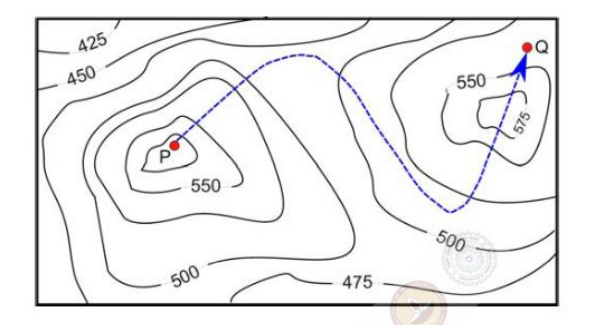
\includegraphics[width=0.5\textwidth]{figures/10.png}
\end{center}
\begin{enumerate}
    \item[(A)] Up-Down-Up-Down  
    \item[(B)] Down-Up-Down-Up  
    \item[(C)] Down-Up-Down  
    \item[(D)] Up-Down-Up  
\end{enumerate}
\vspace{0.5cm}

\section*{Technical Section}

\questiona{Consider \( N \) particles at temperature \( T \), pressure \( P \), volume \( V \) and chemical potential \( \mu \) having energy \( E \). The parameters that are kept constant for a canonical ensemble are}{1}
\begin{enumerate}
    \item[(A)] \( N, V, T \)
    \item[(B)] \( N, V, E \)
    \item[(C)] \( N, P, T \)
    \item[(D)] \( \mu, V, T \)
\end{enumerate}
\vspace{0.5cm}

\questiona{For ortho-hydrogen, the nuclear wavefunction and the rotational quantum number, respectively, are}{2}
\begin{enumerate}
    \item[(A)] antisymmetric and even
    \item[(B)] symmetric and odd
    \item[(C)] symmetric and even
    \item[(D)] antisymmetric and odd
\end{enumerate}
\vspace{0.5cm}

\questiona{\( m_1 \) and \( m_2 \) are the slopes \((\frac{dP}{dT})\) of the solid-liquid equilibrium lines in the P-T phase diagrams of H\(_2\)O and CO\(_2\), respectively. For \( P < 10 \) atm, the values of \( m_1 \) and \( m_2 \) are}{3}
\begin{enumerate}
    \item[(A)] \( m_1 > 0 \) and \( m_2 > 0 \)
    \item[(B)] \( m_1 > 0 \) and \( m_2 < 0 \)
    \item[(C)] \( m_1 < 0 \) and \( m_2 < 0 \)
    \item[(D)] \( m_1 < 0 \) and \( m_2 > 0 \)
\end{enumerate}
\vspace{0.5cm}

\questiona{The rate constant of a reaction is \( 1.25 \times 10^7 \) mol L\(^{-1}\) s\(^{-1}\). If the initial concentration of the reactant is 0.250 mol L\(^{-1}\), the total time (in seconds) required for complete conversion is \_\_\_\_\_\_}{4}
\vspace{0.5cm}

\questiona{Consider an ideal gas of volume \( V \) at temperature \( T \) and pressure \( P \). If the entropy of the gas is \( S \), the partial derivative \( \left( \frac{\partial P}{\partial S} \right)_V \) is equal to}{5}
\begin{enumerate}
    \item[(A)] \( \left( \frac{\partial T}{\partial P} \right)_S \)
    \item[(B)] \( \left( \frac{\partial T}{\partial V} \right)_S \)
    \item[(C)] \( - \left( \frac{\partial T}{\partial V} \right)_S \)
    \item[(D)] \( \left( \frac{\partial T}{\partial S} \right)_V \)
\end{enumerate}
\vspace{0.5cm}

\questiona{The wavelength associated with a particle in one-dimensional box of length \( L \) is ( \( n \) refers to the quantum number)}{6}
\begin{enumerate}
    \item[(A)] \( 2L/n \)
    \item[(B)] \( L/n \)
    \item[(C)] \( nL \)
    \item[(D)] \( L2n \)
\end{enumerate}
\vspace{0.5cm}

\questiona{The dependence of rate constant \( k \) on temperature \( T \) (in K) of a reaction is given by the expression: \\ \[ \ln k = \left( \frac{-5000~K}{T} \right) + 10 \] \\ The activation energy of the reaction (in kJ mol\(^{-1}\)) is \_\_\_\_\_\_ (up to two decimal places)}{7}
\vspace{0.5cm}

\questiona{The lowest energy of a quantum mechanical one-dimensional simple harmonic oscillator is 300 cm\(^{-1}\). The energy (in cm\(^{-1}\)) of the next higher level is \_\_\_\_\_\_}{8}
\vspace{0.5cm}

\questiona{The electronic ground state term for the chromium ion in [Cr(CN)\(_6\)]\(^{4-}\) is}{9}
\begin{enumerate}
    \item[(A)] \( ^3F \)
    \item[(B)] \( ^3H \)
    \item[(C)] \( ^3G \)
    \item[(D)] \( ^5D \)
\end{enumerate}
\vspace{0.5cm}

\questiona{The $VO_4^{3-}, CrO_4^{2-} and MnO_4^{-}$ ions exhibit intense ligand to metal charge transfer transition. The wavelengths of this transition follow the order}{10}
\begin{enumerate}
    \item[(A)] CrO\(_4^{2-}\) < VO\(_4^{3-}\) < MnO\(_4^-\)
    \item[(B)] MnO\(_4^-\) < VO\(_4^{3-}\) < CrO\(_4^{2-}\)
    \item[(C)] VO\(_4^{3-}\) < CrO\(_4^{2-}\) < MnO\(_4^-\)
    \item[(D)] CrO\(_4^{2-}\) < MnO\(_4^-\) < VO\(_4^{3-}\)
\end{enumerate}
\vspace{0.5cm}

\questiona{The lanthanide ion that exhibits color in aqueous solution is}{11}
\begin{enumerate}
    \item[(A)] La(III)
    \item[(B)] Eu(II)
    \item[(C)] Gd(II)
    \item[(D)] Lu(III)
\end{enumerate}
\vspace{0.5cm}

\questiona{The hapticity of cycloheptatriene, $(C_7H_S), in Mo(C_7H_S)(CO)_3$ is \_\_\_\_\_\_ }{12}
\vspace{0.5cm}

\questiona{The V–O–O resonance Raman stretching frequency (in cm\(^{-1}\)) of the O\(_2\) coordinated to iron centre in oxy-hemoglobin is nearly}{13}
\begin{enumerate}
    \item[(A)] 1100
    \item[(B)] 850
    \item[(C)] 1550
    \item[(D)] 1950
\end{enumerate}
\vspace{0.5cm}

\questiona{The energy band diagram for magnesium is \\ 
(The hatched and unhatched regions in the figure correspond to filled and unfilled regions of the band, respectively.)}{14}
\begin{center}
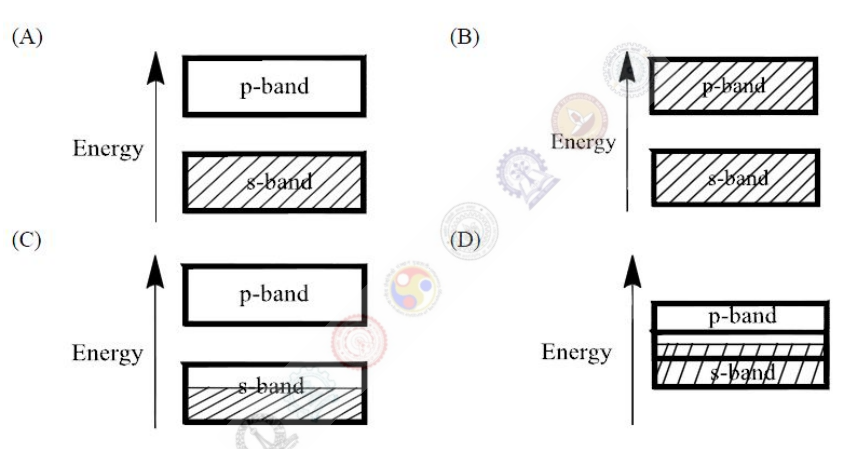
\includegraphics[width=0.8\textwidth]{figures/14.png}
\end{center}

\vspace{0.5cm}

\questiona{P, F and I represent primitive, face-centered and body-centered lattices, respectively. The lattice types of NaCl and CsCl, respectively, are}{15}
\begin{enumerate}
    \item[(A)] F and I
    \item[(B)] F and P
    \item[(C)] I and P
    \item[(D)] P and I
\end{enumerate}
\vspace{0.5cm}

\questiona{The characteristic feature of an electron spin resonance (ESR) spectrum of frozen aqueous solution of CuSO\(_4\)·5H\(_2\)O at 77 K is}{16}
\begin{enumerate}
    \item[(A)] \( g_{\parallel} > g_{\perp} \)
    \item[(B)] \( g_{\parallel} < g_{\perp} \)
    \item[(C)] \( g_{\parallel} = g_{\perp} \)
    \item[(D)] $ g_{x} != g_y != g_Z$
\end{enumerate}
\vspace{0.5cm}

\questiona{The most suitable reagent for the following transformation is}{17}
\begin{center}
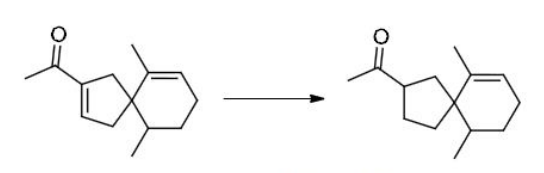
\includegraphics[width=0.5\textwidth]{figures/17.png}
\end{center}
\begin{enumerate}
    \item[(A)] Li / Liq. NH\(_3\)
    \item[(B)] PtO\(_2\) / H\(_2\)
    \item[(C)] LiAlH\(_4\)
    \item[(D)] B\(_2\)H\(_6\)
\end{enumerate}
\vspace{0.5cm}

\questiona{The major products M and N formed in the following reactions are}{18}
\begin{center}
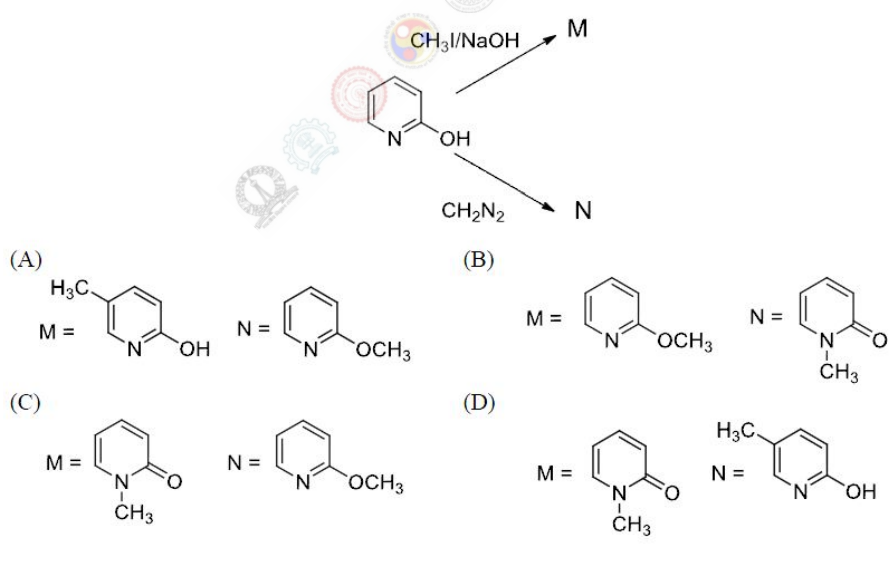
\includegraphics[width=0.9\textwidth]{figures/18.png}
\end{center}

\vspace{0.5cm}

\questiona{The \(^{13}\)C NMR spectrum of acetone-d\(_6\) has a signal at 30 ppm as a septet in the intensity ratio}{19}
\begin{enumerate}
    \item[(A)] 1:6:15:20:15:6:1
    \item[(B)] 1:8:6:1:6:3:1
    \item[(C)] 1:2:3:5:8:3:2
    \item[(D)] 5:15:10:5:1:5:4
\end{enumerate}
\vspace{0.5cm}

\questiona{The major product formed in the following reaction is}{19}
\begin{center}
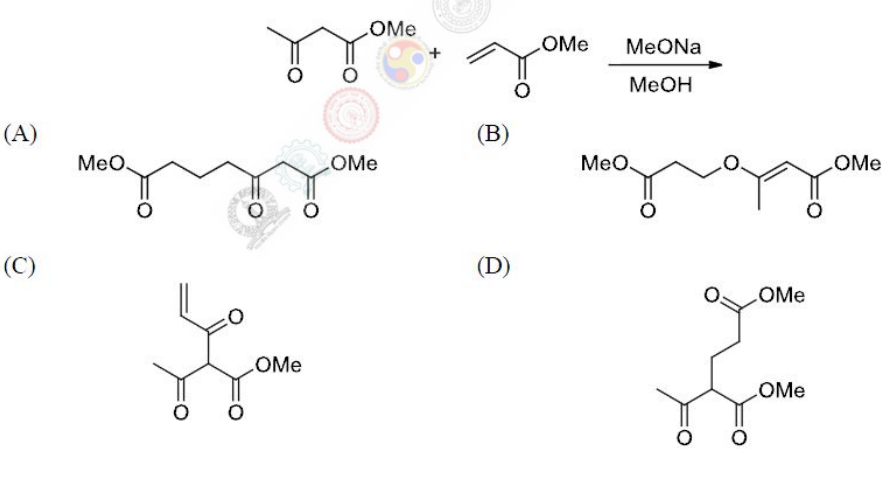
\includegraphics[width=0.9\textwidth]{figures/20.png}
\end{center}

\vspace{0.5cm}

\questiona{The major product obtained in the following reaction is}{21}
\begin{center}
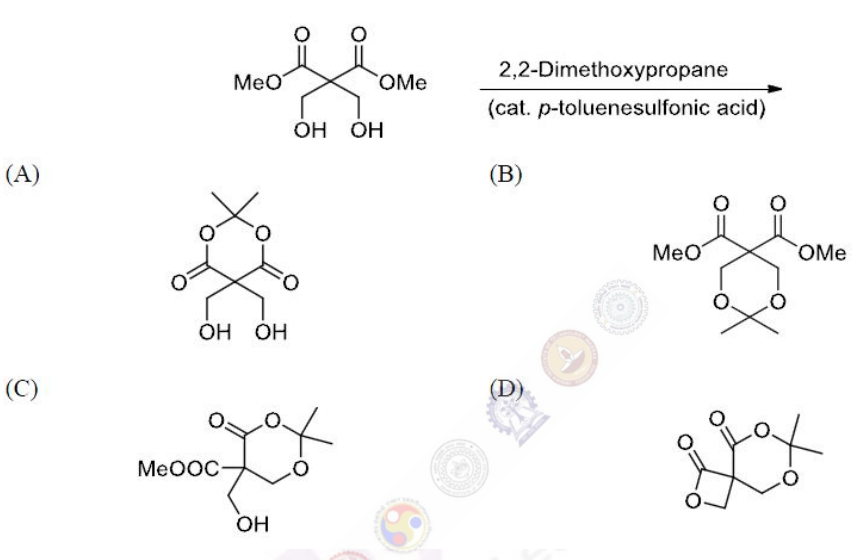
\includegraphics[width=0.9\textwidth]{figures/21.png}
\end{center}

\vspace{0.5cm}

\questiona{In the two-step reaction sequence given below, the starting bis-sulfone acts as}{22}
\begin{center}
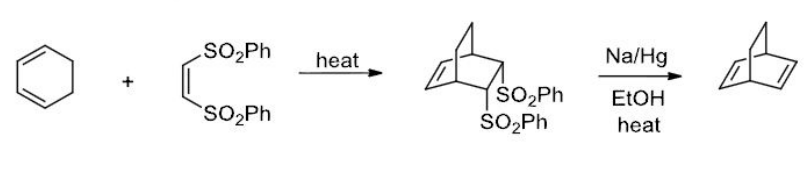
\includegraphics[width=0.8\textwidth]{figures/22.png}
\end{center}
\begin{enumerate}
    \item[(A)] a dienophile and synthetic equivalent of acetylene
    \item[(B)] a dienophile and synthetic equivalent of ethylene
    \item[(C)] a dipolarophile and synthetic equivalent of acetylene
    \item[(D)] a dipolarophile and synthetic equivalent of ethylene
\end{enumerate}
\vspace{0.5cm}

\questiona{The major product formed in the following photochemical reaction is}{23}
\begin{center}
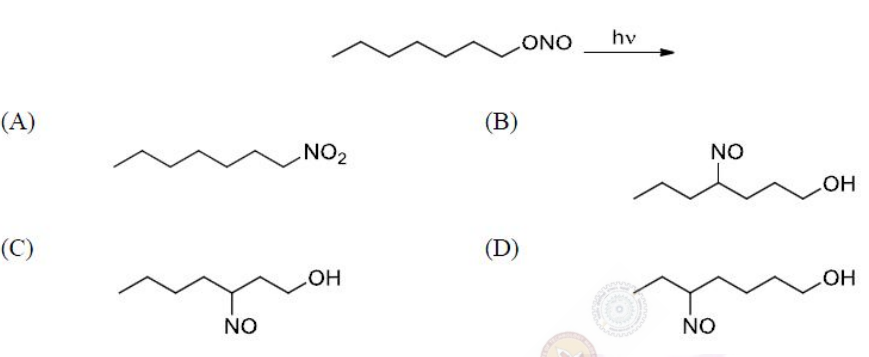
\includegraphics[width=0.9\textwidth]{figures/23.png}
\end{center}
\vspace{0.5cm}

\questiona{The product formed in the following reaction is}{24}
\begin{center}
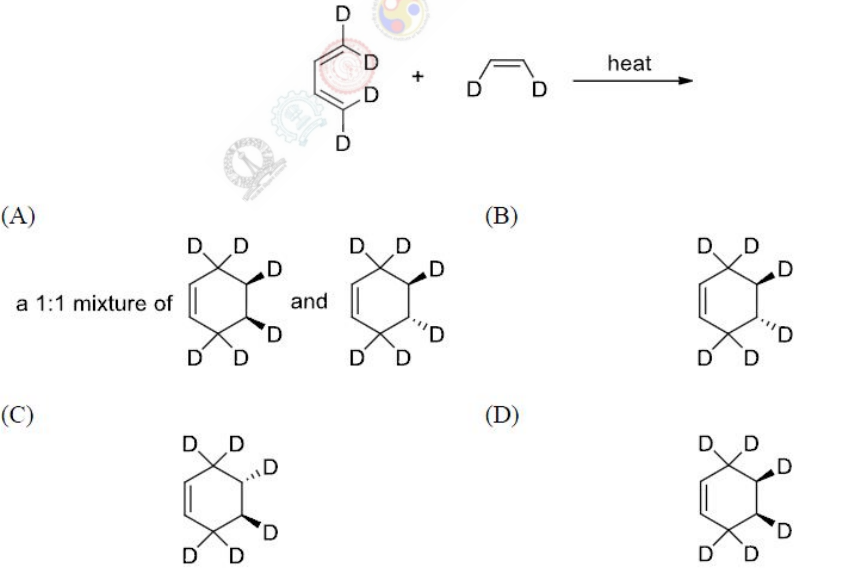
\includegraphics[width=0.9\textwidth]{figures/24.png}
\end{center}
\vspace{0.5cm}

\questiona{The number of possible stereoisomers for cyclononene is \_\_\_\_\_\_}{25}
\vspace{0.5cm}

\questionb{The mobility of a univalent ion in aqueous solution is \( 6.00 \times 10^{-8} \) m\(^2\) s\(^{-1}\) V\(^{-1}\) at 300 K. Its diffusion coefficient at 300 K is \( X \times 10^{-9} \) m\(^2\) s\(^{-1}\). The value of \( X \) is \_\_\_\_\_\_ (up to two decimal places)}{26}
\vspace{0.5cm}

\questionb{For the following consecutive first order reactions \[ X \xrightarrow{k_1=20~s^{-1}} Y \xrightarrow{k_2=0.1~s^{-1}} Z \] the time (in seconds) required for Y to reach its maximum concentration (assuming only X is present at time \( t = 0 \)) is \_\_\_\_\_\_ (up to two decimal places)}{27}
\vspace{0.5cm}

\questionb{Under physiological conditions, the conversion of CO\(_2\) to bicarbonate ion by carbonic anhydrase enzyme (MW = 30,000 g mol\(^{-1}\)) has a turnover number of \( 4.00 \times 10^6 \) s\(^{-1}\). The minimum amount of enzyme (in \(\mu\)g) required to convert 0.44 g of CO\(_2\) to bicarbonate ions in 100 seconds is \_\_\_\_\_\_ (up to two decimal places)}{28}
\vspace{0.5cm}

\questionb{Assume 1,3,5-hexatriene to be a linear molecule and model the \(\pi\) electrons as particles in a one-dimensional box of length 0.70 nm. The wavelength (in nm) corresponding to the transition from the ground-state to the first excited-state is \_\_\_\_\_\_}{29}
\vspace{0.5cm}

\questionb{The standard Gibbs free energy change of the reaction shown below is –2.7 kJ mol\(^{-1}\). \[ \text{Sn(s)} + \text{Pb}^{2+} \rightarrow \text{Sn}^{2+} + \text{Pb(s)} \] Given that \( E^\circ(\text{Pb}^{2+}/\text{Pb}) \) is –0.126 V, the value of \( E^\circ(\text{Sn}^{2+}/\text{Sn}) \) in V is \_\_\_\_\_\_ (up to two decimal places)}{30}
\vspace{0.5cm}

\questionb{The dissociative chemisorption of X\(_2\)(g) on a metal surface follows Langmuir adsorption isotherm. The ratio of the rate constants of the adsorption and desorption processes is 4.0 atm\(^{-1}\). The fractional surface coverage of X (adsorbed) at 1.0 atm pressure is \_\_\_\_\_\_ (up to two decimal places)}{31}
\vspace{0.5cm}

\questionb{The ionic activity coefficients of Ca\(^{2+}\) and F\(^{-}\) are 0.72 and 0.28, respectively. The mean activity coefficient of CaF\(_2\) is \_\_\_\_\_\_ (up to two decimal places)}{32}
\vspace{0.5cm}

\questionb{The angle of orientation (in degrees) of the angular momentum vector with respect to z-axis for \( l = 2 \) and \( m_l = +2 \) state of H-atom is \_\_\_\_\_\_ (up to two decimal places)}{33}
\vspace{0.5cm}

\questionb{The Gibbs free energy of mixing is denoted as \( \Delta G_{mix} \). 1.0 mole of He, 3.0 moles of Ne and 2.0 moles of Ar are mixed at the same pressure and temperature. Assuming ideal gas behavior, the value of \( \Delta G_{mix}/RT \) is \_\_\_\_\_\_ (up to two decimal places)}{34}
\vspace{0.5cm}

\questionb{\( \psi = [c\phi_1 - (1/\sqrt{3})\phi_2] \) represents a normalized molecular orbital constructed from two different atomic orbitals \( \phi_1 \) and \( \phi_2 \) that form an orthonormal set. The value of \( |c| \) is \_\_\_\_\_\_ (up to two decimal places)}{35}\\ \\
\vspace{0.5 cm}
\vspace{0.5cm}
\questionb{In cyclophosphazenes, (NPX\(_2\))\(_3\) (X = F, Cl, Br and Me), the strength of P–N \(\pi\)-bond varies with X in the order}{36}
\begin{enumerate}
    \item[(A)] $F > Cl > Br > Me$
    \item[(B)] $Me > F > Cl > Br$
    \item[(C)] $Br > Cl > F > Me$
    \item[(D)] $Me > Br > Cl > F$
\end{enumerate}
\vspace{0.5cm}

\questionb{The structure type and shape of the polyhedral (skeletal) framework of the carborane, Me\(_2\)C\(_2\)B\(_{10}\)H\(_{10}\), respectively, are}{37}
\begin{enumerate}
    \item[(A)] nido and dodecahedron
    \item[(B)] closo and icosahedron
    \item[(C)] nido and icosahedron
    \item[(D)] closo and dodecahedron
\end{enumerate}
\vspace{0.5cm}

\questionb{If \( \Delta_o \) is the octahedral splitting energy and \( P \) is the electron pairing energy, then the crystal-field stabilization energy (CFSE) of [Co(NH\(_3\))\(_6\)]\(^{2+}\) is}{38}
\begin{enumerate}
    \item[(A)] –0.8\(\Delta_o\) + 2P
    \item[(B)] –0.8\(\Delta_o\) + 1P
    \item[(C)] –0.8\(\Delta_o\)
    \item[(D)] –1.8\(\Delta_o\) + 3P
\end{enumerate}
\vspace{0.5cm}

\questionb{The rates of substitution for the following reaction vary with L in the order\\
\begin{center}
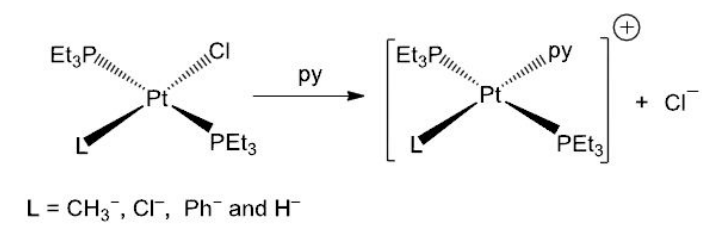
\includegraphics[width=0.8\textwidth]{figures/39.png}
\end{center}}{39}
\begin{enumerate}
    \item[(A)] $CH_3^- > Cl^- > Ph^- > H^-$
    \item[(B)] $Cl^- > Ph^- > H^- > CH_3^-$
    \item[(C)] $Ph^- > CH_3^- > H^- > Cl^-$
    \item[(D)] $H^- > CH_3^- > Ph^- > Cl^-$
\end{enumerate}
\vspace{0.5cm}

\questionb{The product formed in the reaction of MeMn(CO)\(_5\) with \(^{13}\)CO is}{40}
\begin{enumerate}
    \item[(A)] Me(\(^{13}\)CO)Mn(CO)\(_5\)
    \item[(B)] MeCO)Mn(CO)\(_5\)
    \item[(C)] (MeCO)Mn(CO)\(_4\)(\(^{13}\)CO)
    \item[(D)] Me(\(^{13}\)CO)Mn(CO)\(_4\)(\(^{13}\)CO)
\end{enumerate}
\vspace{0.5cm}

\questionb{For the following three alkenes, 1, 2 and 3, the rates of hydrogenation using Wilkinson's catalyst at 25\(^\circ\)C vary in the order}{41}
\begin{center}
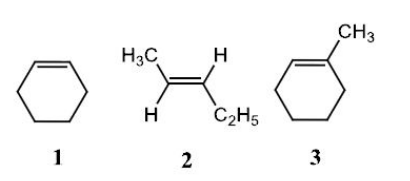
\includegraphics[width=0.5\textwidth]{figures/41.png}
\end{center}
\begin{enumerate}
    \item[(A)] $1 > 3 > 2$
    \item[(B)] $1 > 2 > 3$
    \item[(C)] $2 > 1 > 3$
    \item[(D)] $2 > 3 > 1$
\end{enumerate}
\vspace{0.5cm}

\questionb{\(^{219}\)Bi undergoes \(\beta^-\) decay to \(\frac{1}{8}\) of its initial amount in 15 days. The time required for its decay to \(\frac{1}{64}\) of its initial amount is \_\_\_\_\_\_ days (up to two decimal places)}{42}
\vspace{0.5cm}

\questionb{The metal ion and the macrocyclic skeleton present in the green pigment of plants, respectively, are}{43}
\begin{enumerate}
    \item[(A)] Mg(II) and chlorin
    \item[(B)] Mg(II) and corrin
    \item[(C)] Mn(II) and chlorin
    \item[(D)] Mg(II) and porphine
\end{enumerate}
\vspace{0.5cm}

\questionb{The spinel structure of MgAl\(_2\)O\(_4\) has cubic close packed arrangement of oxide ions. The fractions of the octahedral and tetrahedral sites occupied by cations, respectively, are}{44}
\begin{enumerate}
    \item[(A)] \(\frac{1}{2}\) and \(\frac{1}{8}\)
    \item[(B)] \(\frac{1}{4}\) and \(\frac{1}{2}\)
    \item[(C)] \(\frac{1}{8}\) and \(\frac{1}{4}\)
    \item[(D)] \(\frac{1}{2}\) and \(\frac{1}{4}\)
\end{enumerate}
\vspace{0.5cm}

\questionb{The diffusion limiting current (\(i_d\)) at a dropping mercury electrode for an aqueous Mg(II) solution of concentration \( c \) (mol L\(^{-1}\)) is 300 \(\mu\)A. If \( c \) is increased by 0.1 mol L\(^{-1}\), \( i_d \) increases to 900 \(\mu\)A. The value of \( c \) (in mol L\(^{-1}\)) is \_\_\_\_\_\_ (up to two decimal places)}{45}
\vspace{0.5cm}

\questionb{The major product formed in the following reaction is}{46}
\begin{center}
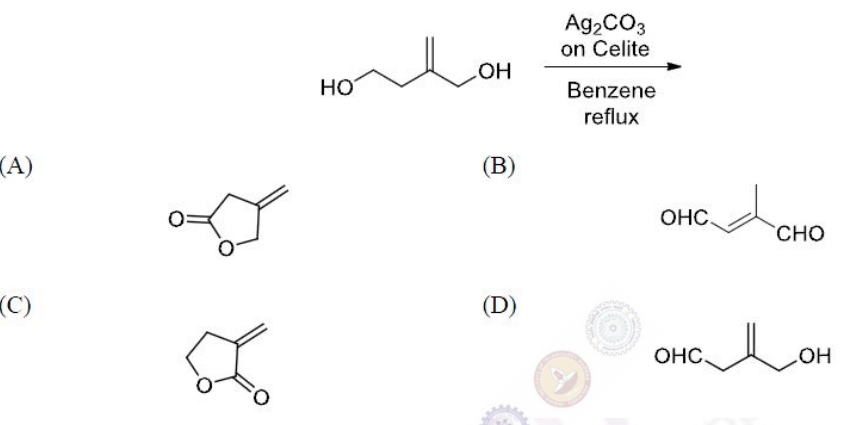
\includegraphics[width=0.9\textwidth]{figures/46.png}
\end{center}

\vspace{0.5cm}

\questionb{The product formed in the following photochemical reaction is}{47}
\begin{center}
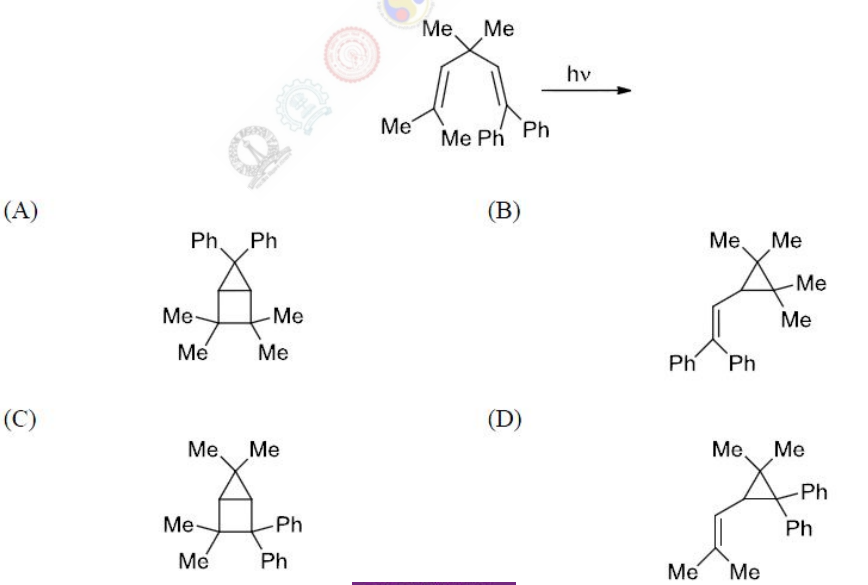
\includegraphics[width=0.9\textwidth]{figures/47.png}
\end{center}
\vspace{0.5cm}

\questionb{Among the following decahydroquinoline toluenesulfonates (Ts), the one that yields 9-methylamino-E-non-5-enal as a major product upon aqueous solvolysis is}{48}
\begin{center}
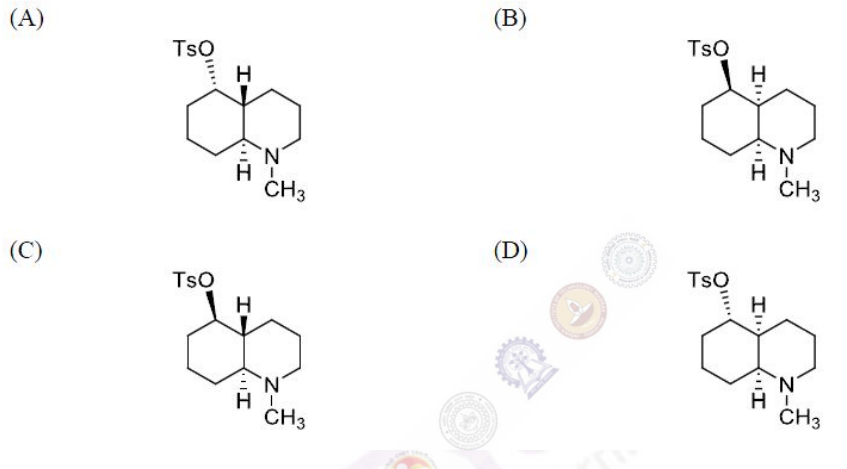
\includegraphics[width=0.9\textwidth]{figures/48.png}
\end{center}
\vspace{0.5cm}

\questionb{The product obtained in the following solvolysis reaction is}{49}
\begin{center}
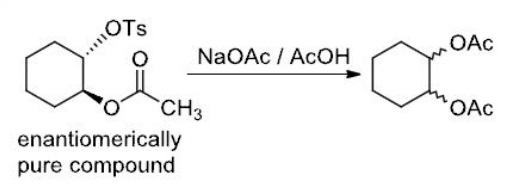
\includegraphics[width=0.5\textwidth]{figures/49.png}
\end{center}
\begin{enumerate}
    \item[(A)] a racemic mixture of trans 1,2-diacetoxycyclohexane
    \item[(B)] enantiomerically pure trans 1,2-diacetoxycyclohexane
    \item[(C)] racemic cis 1,2-diacetoxycyclohexane
    \item[(D)] a mixture of cis and trans 1,2-diacetoxycyclohexane
\end{enumerate}
\vspace{0.5cm}

\questionb{The spectroscopic data for an organic compound with molecular formula C\(_{10}\)H\(_{12}\)O\(_2\) are given below. \\
IR band around 1750 cm\(^{-1}\); \( ^1 \)H NMR: 7.3 (m, 5H), 5.85 (q, 1H, J = 7.2 Hz), 2.05 (s, 3H), 1.5 (d, 3H, J = 7.2 Hz) ppm. \\
The compound is}{50}
\begin{enumerate}
    \item[(A)] methyl 2-phenylpropionate
    \item[(B)] 1-(phenylethyl) acetate
    \item[(C)] 2-(phenylethyl) acetate
    \item[(D)] methyl 3-phenylpropionate
\end{enumerate}
\vspace{0.5cm}

\questionb{The structures of the intermediate [P] and major product [Q] formed in the following reaction sequence are}{51}
\begin{center}
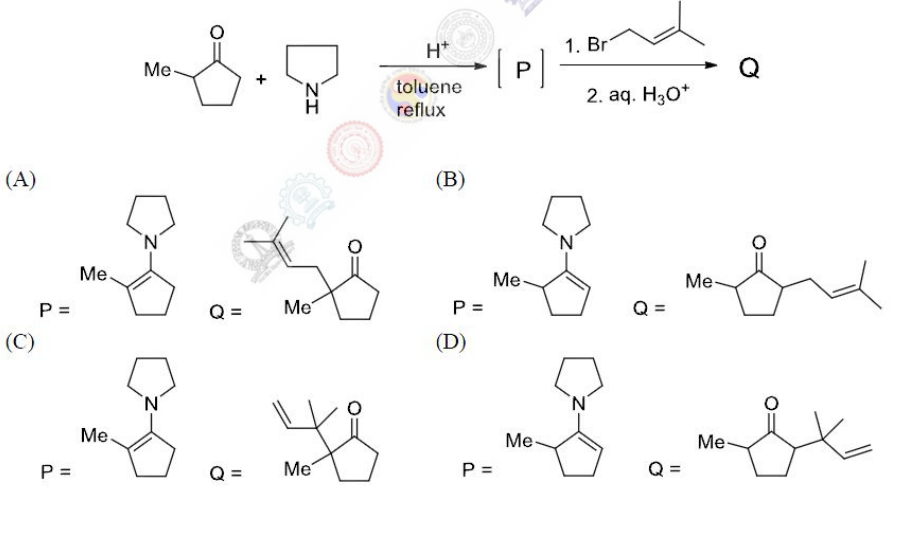
\includegraphics[width=0.9\textwidth]{figures/51.png}
\end{center}
\vspace{0.5cm}

\questionb{Hydration of fumaric acid gives malic acid as shown below. Assume that addition of water takes place specifically from A face or B face. The correct statement pertaining to stereochemistry of malic acid formed is}{52}
\begin{center}
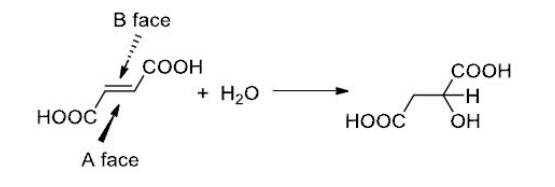
\includegraphics[width=0.5\textwidth]{figures/52.png}
\end{center}
\begin{enumerate}
    \item[(A)] addition specifically from A face gives S isomer of malic acid
    \item[(B)] addition specifically from B face gives S isomer of malic acid
    \item[(C)] addition specifically from A face gives R isomer of malic acid
    \item[(D)] addition specifically from B face gives a racemic mixture of malic acid
\end{enumerate}
\vspace{0.5cm}

\questionb{Hydroboration of 2-butyne with (C\(_8\)H\(_{11}\))\(_2\)BH yields the intermediate [U], which on treatment with I\(_2\) and NaOMe at –78 °C, gives product [V]. The structures of U and V are}{53}
\begin{center}
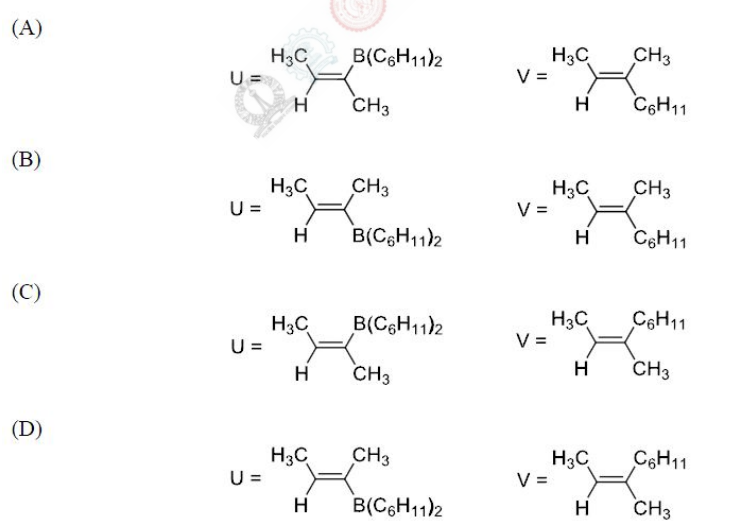
\includegraphics[width=0.8\textwidth]{figures/53.png}
\end{center}
\vspace{0.5cm}

\questionb{The structures of the major products [W] and [X] in the following synthetic scheme are}{54}
\begin{center}
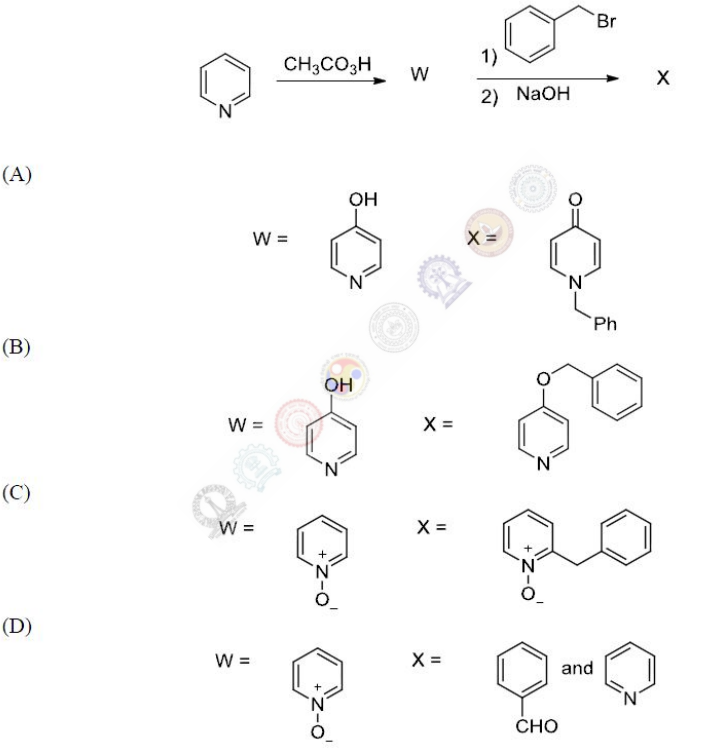
\includegraphics[width=0.7\textwidth]{figures/54.png}
\end{center}
\vspace{0.5cm}

\questionb{The major products [Y] and [Z] in the following reaction sequence are}{55}
\begin{center}
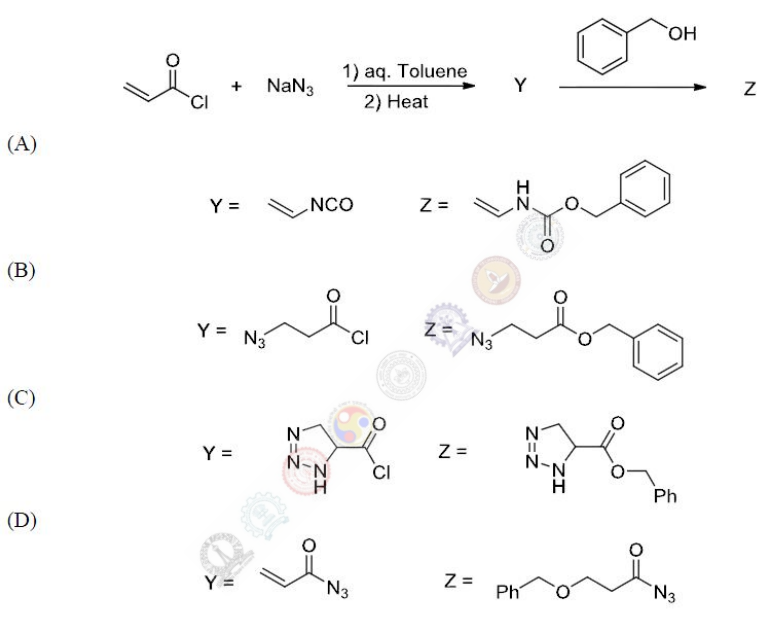
\includegraphics[width=0.9\textwidth]{figures/55.png}
\end{center}

\vspace{0.5cm}



\vspace{5cm}
\begin{center}
\textbf{END OF THE QUESTION PAPER} \\
\rule{\textwidth}{0.5pt} 
\end{center}

\end{document}
